\newpage
\thispagestyle{sectioned}

\appendix

%%%%%%%%%%%%%%%%%%%%%%%%%%%%%%%%%%%%%%%%%%%%%%%%%%%%%%%%%%%%%%%%%%%%
%%%%%%%%%%%%%%%%%%%%%%%%%%%%% APPEND A %%%%%%%%%%%%%%%%%%%%%%%%%%%%%
%%%%%%%%%%%%%%%%%%%%%%%%%%%%%%%%%%%%%%%%%%%%%%%%%%%%%%%%%%%%%%%%%%%%

\chapter{Migración de SwellRT a Android: Aspectos Técnicos}
 	
	Existe un problema con la construcción y depuración del código de SwellRT en Eclipse. Android \textbf{limita el número de métodos máximos de una aplicacion a 65K} \cite{ref:android_limit65k} por cuestiones de eficiencia. Para evitar esta limitación, durante el proceso de construcción el SDK de Android utiliza, entre otras, una herramienta llamada \textbf{ProGuard} \cite{ref:android_proguard}. Esta herramienta se encarga de optimizar el código de la aplicacion buscando remover clases que no se utilizan y ofuscando el código para prevenir la ingeniería inversa. En el caso de SwellRT, el código posee un gran número de clases java necesarias para desplegar el servidor y el cliente de la herramienta, por lo que es necesaria dicha optimización de código realizada por ProGuard. El sistema de compilación de aplicaciones de Android tiene dos formas: compilación de la aplicación en modo debug (para hacer pruebas cuando todavía se encuentra en fase de desarrollo) y en modo release (la aplicación se encuentra en su versión final y se empaqueta y se firma digitalmente para lanzarla al público). En el caso de Eclipse, ProGuard solo se ejecuta cuando se construye en modo release, por lo que cuando se intenta compilar una aplicación con tantas clases como SwellRT mientras se desarrolla (modo debug) el sistema da error y no se puede compilar el código para probarlo en el emulador.

	La solución que se encontró fue desarrollar en Eclipse (por las facilidades que el entorno proporciona para escribir código) pero realizar el proceso de construcción del código por consola de comandos, ya que en este caso sí que se puede compilar la aplicación en modo debug utilizando ProGuard.

\section{Proceso de Construcción por Consola}

		Para construir la aplicación por consola de comandos, Android utiliza la herramienta Apache Ant \cite{ref:ant} para automatizar el proceso de construcción \cite{ref:android_cmd_line}. Es importante asimismo tener definida la variable de entorno JAVA\_HOME con la ruta de acceso al JDK de java instalado en la máquina. Conviene también, por comodidad a la hora de trabajar con la consola, añadir al PATH del sistema las rutas a la carpeta donde esta el SDK de android (/sdk) y dentro de esta ruta añadir asimismo rutas a las carpetas /tools y /platform-tools. 

Existen dos formas de realizar la construcción en modo debug de una app:  

\textbf{1 - Sin tener previamente lanzado un emulador o conectado al ordenador un dispositivo android en modo debug \cite{ref:android_device_setUp}:} 
 
 	 En este caso es necesario construir la aplicación y luego lanzar el emulador para después instalar la aplicación en él. Para construir la aplicacion en modo debug,  estando en la carpeta raíz de nuestro proyecto y ejecutando el siguiente comando: 

 	 \begin{lstlisting}[style=console, numbers=none]
		$ ant clean debug
	 \end{lstlisting}
 	 
 	 Esto generará una aplicacion instalable en el directorio /bin del proyecto bajo el formato que Android usa para sus aplicaciones (.apk). El siguiente paso es ejecutar un emulador o conectar un dispositivo android por USB. Para ejecutar un emulador, abrimos otra consola y utilizamos el siguiente comando:
 	 
 	 \begin{lstlisting}[style=console, numbers=none]
		$ android avd
	 \end{lstlisting}
 	 
 	 Lo que despliega la herramienta Android Virtual Device Manager (Ver Sección \ref{sssec:eclipse}) para elegir/crear el emulador que se quiera ejecutar. Se pueden elegir multitud de parámetros \cite{ref:android_avd_params} para el dispositivo que emula (resolución y tamaño de pantalla, de memoria Ram, elementos hardware emulados, etcétera.) siendo lo más importante elegir un API (versión de Android) que se corresponda con el API que se haya elegido para la aplicación (en este caso API 19). Es recomendable también elegir una imagen del sistema que use un procesador con arquitectura Intel x86, ya que si se elige la opción por defecto de ARM (los dispositivos móviles actuales usan procesadores ARM) la ejecución del emulador se ralentiza mucho al tener que emular una arquitectura de procesador distinta a la suya (los ordenadores actuales usan arquitectura Intel x86 en su mayoría). Esto únicamente afecta al rendimiento del emulador, la aplicación es independiente de la arquitectura que haya por debajo. \\[.2cm]
 
     Una vez lanzado el emulador/dispositivo móvil, se procede a instalar la aplicación en él ejecutando el siguiente comando en la primera consola (en la que se construyó la aplicación):
		      	 
 	 \begin{lstlisting}[style=console, numbers=none]
		$ adb install XXXX.apk
	 \end{lstlisting}		
 	 
 	 Siendo XXXX la ruta a donde se encuentra el .apk de la aplicación que previamente se ha construido (/bin). La herramienta ADB (Android Debug Bridge) \cite{ref:android_adb} es la que permite la comunicación entre el proceso de la consola de comandos y el emulador/dispositivo móvil. Es importante destacar que si se tienen varios emuladores/dispositivos móviles en ejecución/conectados hay que especificar en cual se quiere instalar la aplicación añadiendo al comando lo siguiente: \textbf{-s emulator -YYYY} siendo esto último el identificador del emulador que podemos encontrar en el título de la ventana del emulador. 
	     
	\begin{figure}[H]
      \centering
	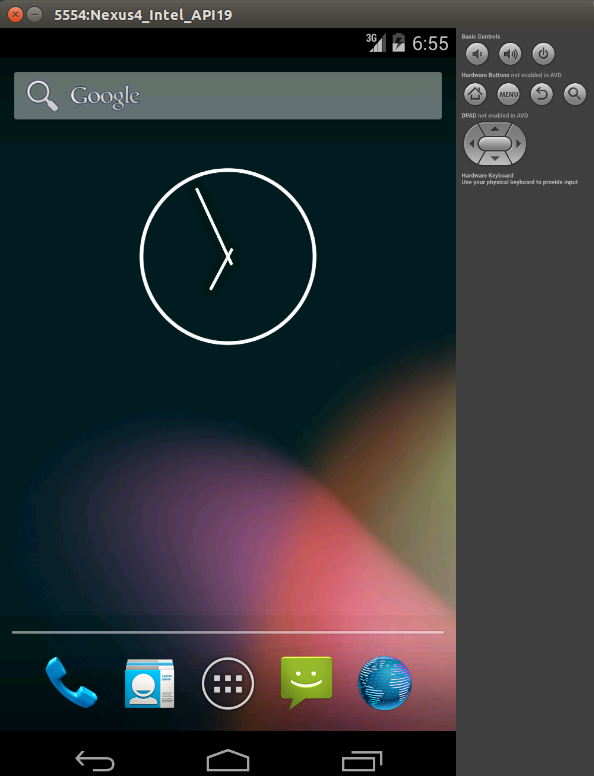
\includegraphics[keepaspectratio, scale=0.3]{Media/Captures/emulator_api_19.png}
      \caption{Emulador Android API 19}
      \label{fig:android_emulator19}
    \end{figure} 
    
    De esta manera se puede probar la aplicación, que será lanzada en el emulador/dispositivo una vez termine su instalación. 

	\textbf{2 - Teniendo un emulador previamente lanzado (ver sección anterior para ver cómo se lanza) o un dispositivo móvil ya conectado por USB:} \
	
	En este caso es todavía más sencillo el proceso de construcción. Estando en la carpeta raíz del proyecto se puede compilar e instalar la aplicación con un solo comando:

 	 \begin{lstlisting}[style=console, numbers=none]
		$ ant debug install
	\end{lstlisting}	
 	 
 	 Es importante destacar que este comando solo funciona si se tiene un único emulador o dispositivo conectado, de lo contrario habrá que utilizar el método anterior. 

    
\section{Proceso de Depuración} \label{sec:debug}
    
    Una vez instalada una aplicación, se puede depurar su código en ejecución usando la herramienta DDMS del ADT en conjunto con la vista de Debug de Eclipse. Pero antes hay que especificar qué aplicación queremos depurar de las que puedan estar instaladas en el dispositivo o emulador. 

En el caso del emulador se debe lanzar la aplicación llamada “Dev Tools” y abrir el menú “Developer Options”. Dentro de este menú habilitaremos las opciones de “USB debugging” y de  “Wait for debugger”. Se pulsará sobre “Select Debug app” y se seleccionará la aplicación que se quiera depurar. 

En el caso de un dispositivo Android se debe ir a los Ajustes del dispositivo y seleccionar el menú de Opciones de Desarrollador. Aquí se habilitan las opciones de "Depuración de USB"  (si no están habilitadas ya) y de "Esperar al depurador". Se pulsa donde pone "Seleccione una aplicación para depurar" y se elige la aplicación que se quiera depurar. 

Una vez hecho esto, cada vez que se jecute la aplicacion saldrá un mensaje de advertencia y se quedará esperando a que se conecte un depurador para continuar con su ejecución. Para esto, en Eclipse se abre la vista de DDMS. Aquí aparecerá, entre otras cosas, un espacio con todos los procesos en ejecución en el dispositivo/emulador. Se localiza el proceso de nuestra aplicación y se pulsa sobre el ''escarabajo'' verde para conectar el depurador a ella. Llegados a este punto la aplicacion continua su ejecución en el emulador y aparece un escarabajo verde al lado del proceso de la app en la ventana de DDMS, que indica que se esta depurando ese proceso. Es entonces cuando se puede abrir la vista de depuración de Eclipse y proceder a trabajar con breakpoints para depurar y estudiar el código con el fin de solucionar errores.


%%%%%%%%%%%%%%%%%%%%%%%%%%%%%%%%%%%%%%%%%%%%%%%%%%%%%%%%%%%%%%%%%%%%
%%%%%%%%%%%%%%%%%%%%%%%%%%%%% APPEND B %%%%%%%%%%%%%%%%%%%%%%%%%%%%%
%%%%%%%%%%%%%%%%%%%%%%%%%%%%%%%%%%%%%%%%%%%%%%%%%%%%%%%%%%%%%%%%%%%%


\chapter{Listados de Código Fuente}

En este apéndice se recogen solo algunos fragmentos de código que se estiman representativos para complementar la información que se expone a lo largo de todo este documento. Se recoge código tanto de la Migración de SwellRT a Android, del desarrollo del Servicio Web REST y de la implementación de la aplicación Android.

\section{Migración de Wave a Android: SwellRT}

\subsection{Esquema de conexión HTTP}\label{ssec:codeHTTP}

\lstset{language=Java, breaklines=true, autogobble=true, basicstyle=\ttfamily\footnotesize, commentstyle=\color{OliveGreen}, keywordstyle=\color{MidnightBlue}}
	  \begin{lstlisting}[frame=single]	  
import java.net.HttpURLConnection;

private void login(final String user, final String password, final Callback<String, String> callback) {
  
    //Construct the URL String urlStr with the server, user and password parameters
    URL url = new URL(urlStr); //String 
    HttpURLConnection connection = (HttpURLConnection) url.openConnection(); //Open the connection to the given URL 
    connection.setDoOutput(true); // allow the POST connection
    connection.setRequestProperty("Accept-Charset", CHARSET);
    connection.setRequestProperty("Content-Type", "application/x-www-form-urlencoded;charset=" + CHARSET);

    OutputStream out = connection.getOutputStream(); 
    out.write(queryStr.getBytes(CHARSET)); //Set the POST parameters

    if (connection.getResponseCode() != 200) {
	//ERROR during the connection
	connection.disconnect(); //Disconnect from the server.
    } else {
	//Continue with the login process (WebSocket)
	connection.disconnect(); //Disconnect from the server.
    }		      
}	    
	  \end{lstlisting}  
	  
\subsection{Esquema de conexión con AsyncTask}\label{ssec:codeAsynctask}	  
	  
	  \lstset{language=Java, breaklines=true, autogobble=true, basicstyle=\ttfamily\footnotesize, commentstyle=\color{OliveGreen}, keywordstyle=\color{MidnightBlue}}
	  \begin{lstlisting}[frame=single]
	  
private class LoginTask extends AsyncTask<String, Void, String> {
    
    @Override
    protected String doInBackground(String... params) { //method that executes on the new Thread without blocking the UI Thread
      login(params[0], params[1], params[2]); //Do the login 
      return sessionId //String needed for the WebSocket connection and based on the cookie received from the server.     
    }
   
   @Override
    protected void onPostExecute(String result) { //method that executes on the UI Thread once doInBackground() finishes its execution.    
      
      if (result != null) { 
        callback.onLogin(); //Notify the login success using the proper callback method
        
      } else { //The doInBackGround method has had a problem and the result of its execution was null
        callback.onError("Wave Login Error"); //Notify the login error using the proper callback method      
      }
    }
}    
	  \end{lstlisting} 
	  
\subsection{Esquema de uso de WAsync}\label{ssec:codewAsync}
	  	  
\lstset{language=Java, breaklines=true, autogobble=true, basicstyle=\ttfamily\footnotesize, commentstyle=\color{OliveGreen}, keywordstyle=\color{MidnightBlue}}
	  \begin{lstlisting}[frame=single]	  	  
	  
//Create the atmosphere client
AtmosphereClient client = ClientFactory.getDefault().newClient(AtmosphereClient.class);

//Configure client with URL
AtmosphereRequestBuilder requestBuilder = client.newRequestBuilder()
  .method(Request.METHOD.GET).trackMessageLength(true).uri(WaveSocketWAsync.this.urlBase)
  .transport(Request.TRANSPORT.WEBSOCKET)
  
//Create and configure socket
WaveSocketWAsync.this.socket = client.create(client.newOptionsBuilder().runtime(ahc).build())
  .on(Event.OPEN.name(), new Function<String>() { //Equivalent to GWT onOpen() method
    @Override
    public void on(String arg0) {
		// set the actions to do and call the proper callback function (callback.onConnect())
    }
    
  }).on(Event.CLOSE.name(), new Function<String>() { //Equivalent to GWT onClose() method
    @Override
    public void on(String arg0) {
    // set the actions to do and call the proper callback function (callback.onDisconnect())
    }
    
  }).on(Event.MESSAGE.name(), new Function<String>() {
    @Override
    public void on(String arg) { //Equivalent to GWT onMessage() method
    // set the actions to do and call the proper callback function (callback.onMessage())
    }
    
  }).on(new Function<Throwable>() {
    @Override
    public void on(Throwable t) {
		// catch possible exceptions
    }
  });
          
try {
// connect to the server
socket.open(requestBuilder.build());
} catch (IOException e) {
	// catch possible exceptions
}
      
//send a given message to the server, equivalent to GWT send(msg) method 
socket.fire(Data);
	\end{lstlisting}
	  
\section{Servicio Web REST (Laravel)}

\subsection{Esquema de Rutas Simple}\label{ssec:codeRoutesSimple}

\lstset{
  language        = php}
\begin{lstlisting}[frame=single]
// Posibles operaciones con el objeto "propuesta"
Route::get('/proposal', 'ProposalController@index');
  // Obtiene el listado de todas las propuestas
Route::get('/proposal/{id}', 'ProposalController@show');
  // Obtiene la prupuesta pasada por el campo {id}
Route::post('/proposal', 'ProposalController@create');
  // Crea una nueva propuesta en el servidor
Route::put('/proposal/{id}', 'ProposalController@update');
  // Actualiza la propuesta pasada por {id}
Route::delete('/proposal/{id}', 'ProposalController@destroy');
  // Borra la propuesta pasada por {id}
\end{lstlisting}

\subsection{Esquema de Rutas Agrupadas}\label{ssec:codeRoutesGroupe}

\lstset{
  language        = php}
\begin{lstlisting}[frame=single]
Route::group(['prefix' => 'proposal'], function()
{
    Route::get('/', 'ProposalController@index');
    Route::get('/{id}', 'ProposalController@show');
    Route::post('/', 'ProposalController@create');
    Route::put('/{id}', 'ProposalController@update');
    Route::delete('/{id}','ProposalController@destroy');
});
\end{lstlisting}

\subsection{Esquema de Rutas de Propuestas Agrupadas}\label{ssec:codeRoutesGroupeProposals}

\lstset{
  language        = php}
\begin{lstlisting}[frame=single]
Route::group(['prefix' => 'proposal'], function()
{
  Route::get('/', 'ProposalController@index');
  Route::post('/', 'ProposalController@create');
  Route::group(['prefix' => '/{id}'], function()
  {
    Route::get('/', 'ProposalController@show');
    Route::put('/', 'ProposalController@update');
    Route::delete('/','ProposalController@destroy');
  });
});
\end{lstlisting}

\subsection{Esquema de Controlador de Propuestas}\label{ssec:codeControllerProposals}

\lstset{
  language        = php}
\begin{lstlisting}[frame=single]
<?php namespace App\Http\Controllers;

use App\Http\Requests;
use App\Http\Controllers\Controller;
use DB;

class ProposalController extends Controller {
  /**
  * Display a listing of the resource.
  *
  * @return Response
  */
  public function index()
  {
    return DB::select('SELECT * FROM `proposal`');
  }
}
\end{lstlisting}

\section{Aplicación Android}

\subsection{Función de construcción del árbol de Programa Político}\label{ssec:codeProgramTree}

 \lstset{language=Java, breaklines=true, autogobble=true, basicstyle=\ttfamily\footnotesize, commentstyle=\color{OliveGreen}, keywordstyle=\color{MidnightBlue}}
	  \begin{lstlisting}[frame=single]	
protected int createIndex(Section parent, List<Section> JSONResult, int index) {

    // X = currentSection
    Section currentSection = JSONResult.get(index);

    if (parent.getlSections() == null) {
      parent.setlSections(new ArrayList<Section>());
    }
	    
    parent.addSubSection(currentSection);

    // c = nextIndex
    int nextIndex = index + 1;

    while ((nextIndex < JSONResult.size()) && (getLevel(JSONResult.get(nextIndex)) >= getLevel(currentSection))) {
      
      if (getLevel(JSONResult.get(nextIndex)) == getLevel(currentSection)) {
	currentSection = JSONResult.get(nextIndex);
	nextIndex++;
	parent.addSubSection(currentSection);
	
      } else if (getLevel(JSONResult.get(nextIndex)) > getLevel(currentSection))
	nextIndex = createIndex(currentSection, JSONResult, nextIndex);
    }
    
    return nextIndex;
}

protected int getLevel(Section sec) {
  
  int id_sec = sec.getmSection(), level;
  
  if (id_sec % 100 != 0) {
      level = 4;
      
  } else if (id_sec % 10000 != 0) {
      level = 3;
      
  } else if (id_sec % 1000000 != 0) {
      level = 2;
      
  } else
      level = 1;
      
  return level;
}	   
	  \end{lstlisting}
	  
\subsection{Registrar Usuario en SwellRT} \label{ssec:waveRegister}

 \lstset{language=Java, breaklines=true, autogobble=true, basicstyle=\ttfamily\footnotesize, commentstyle=\color{OliveGreen}, keywordstyle=\color{MidnightBlue}}
	  \begin{lstlisting}[frame=single]	  
public class MainActivity implements ServiceConnection, SwellRTServiceCallback {
	  
	private SwellRTService mSwellRT;	  	  
	protected void bindSwellRTService() {

        if (mSwellRT == null) {
            final Intent mWaveServiceIntent = new Intent(this, SwellRTService.class);
            bindService(mWaveServiceIntent, this, Context.BIND_AUTO_CREATE);
        }
    	}
   		
    	@Override
    protected void onCreate(Bundle savedInstanceState) {
    		//Create view and get view references    		
    		bindSwellRTService(); //Bind to the service  		
    }
    
    //AsyncTask for registering the user.
    public void registerWaveUser() {
        AsyncTask mRegisterTask = new AsyncTask<String, Void, Boolean>() {

       		@Override
        		protected Boolean doInBackground(String... params) {
           		return mSwellRT.registerUser(params[0], params[1], params[2]);
        		}

        		@Override
        		protected void onPostExecute(Boolean result) {
          		if (result)
              		Toast.makeText(MainActivity.this, "User created successfully", Toast.LENGTH_LONG).show();
           		else
              Toast.makeText(MainActivity.this, "Error creating user", Toast.LENGTH_LONG).show();
            }
        };
		
		//Execute task with the server, user and password
        mRegisterTask.execute(WAVE_SERVER, "" + User.ID_USER + "@local.net", "password");
    }

	//Callback called when the service is connected.
    @Override
    public void onServiceConnected(ComponentName name, IBinder service) {
        mSwellRT = ((SwellRTService.SwellRTBinder) service).getService(this);
        Log.d(this.getClass().getSimpleName(), "SwellRT Service Bound");
        
        registerWaveUser(); //Do the register.
    }

    @Override
    public void onServiceDisconnected(ComponentName name) {
        mSwellRT = null;
        Log.d(this.getClass().getSimpleName(), "SwellRT Service unBound");
}	
    
    }
    
	  \end{lstlisting}
	  
\subsection{Crear nueva Wave (Model) en SwellRT} \label{ssec:waveCreateModel}

\lstset{language=Java, breaklines=true, autogobble=true, basicstyle=\ttfamily\footnotesize, commentstyle=\color{OliveGreen}, keywordstyle=\color{MidnightBlue}}
	  \begin{lstlisting}[frame=single]  
public class NewProposalActivity extends SwellRTActivity {
	  
	  @Override
	  protected void onCreate(Bundle savedInstanceState) {
	  	//Get the proposal info from the user view, if there is no ''how'' or ''cost'', create a new wave model.
	  }
	  
	  public void doStartSession() {
        // Open Session with ID_USER
        try {
            mSwellRT.startSession(MainActivity.WAVE_SERVER,
                    "" + User.ID_USER + "@local.net", "password");
        } catch (MalformedURLException e) {
            e.printStackTrace();
        } catch (InvalidParticipantAddress invalidParticipantAddress) {
            invalidParticipantAddress.printStackTrace();
        }
    }

    // SwellRT Service Callbacks
    @Override
    public void onServiceConnected(ComponentName name, IBinder service) {
        mSwellRT = ((SwellRTService.SwellRTBinder) service).getService(this);
        doStartSession();
        Log.d(this.getClass().getSimpleName(), "SwellRT Service Bound");
    }
    
    @Override
    public void onStartSessionSuccess(String session) {		
		getService().createModel();
    }
   
    @Override
    public void onCreate(Model model) {  // Callback called when a model is created.
        
        // Get the Id of the wave/model to store in the database
        WaveId idW = model.getWaveId();
        String idWave = idW.toString();
        String id = "";
        id = idWave.substring(8, idWave.length() - 1);

        //Store the proposal (with the Wave Id) in the database.
        postCollaborativeProposal(id);

        // Create a text document for each Pad
        TextType padHow = model.createText("¿Cómo lo harías?");
        TextType padCost = model.createText("¿Cómo lo financiarias?");

        // Include the document as part of the wave/model in the "root" map.
        if(createHowWave)
            model.getRoot().put("padHow", padHow);
        if(createCostWave)
            model.getRoot().put("padCost", padCost);

        // Allow current user to read/write the text of the Pad
        model.addParticipant("" + User.ID_USER + "@local.net");
    }  	
}	  
	  \end{lstlisting}
	  
\subsection{Abrir Pad colaborativo en SwellRT} \label{ssec:waveOpenPad}
	  
	  

\addcontentsline{toc}{chapter}{\numberline{}Bibliografía} %add bibliography to the index

\rhead{}
\renewcommand{\headrulewidth}{0pt}